\cleardoublepage%
\chapter{\label{chap:res}Results and Discussion}%

%This is where you present your findings. As much as possible, structure your results along the lines of your research questions. Start with the simplest results first and proceed to more complex ones. Tables and Figures should be clear enough that they need little explanation: do not simply re-write the numbers as text to fill space. Rather, highlight trends, outliers, or gaps. 

\section{\label{sec:res_design}Platform and Framework Design} %reference to methods

\begin{figure}[H]
    \centering
    \includegraphics[width=0.5\linewidth]{overleaf/images/placeholder.png}
    \vspace{\ftspace}
    \caption{Platform Architecture}
    \label{fig:ssp_architecture}
\end{figure}

Put in the design and architecture of the platform,


and present the developed GitHub page, layout, website, guides and stuff and its capabilities

\section{\label{sec:res_capabilities}Smart System Platform} %reference to methods

\subsection{\label{sec:res_website}Website}

Website and quick start Guides

the website was to be tested with the Google for Developers PageSpeed Insights, which resulted in an overall score of 100 out of 100 for both mobile and desktop version of the webpage.

\subsection{\label{sec:res_ide}IDE and Network Management}

pyscript page, and perhaps mention the AI idea and other stuff

\subsection{\label{sec:res_hardware}Hardware}

Module approach

Future board

etc.

\begin{figure}[H]
    \centering
    \includegraphics[width=0.5\linewidth]{overleaf/images/placeholder.png}
    \vspace{\ftspace}
    \caption{Hardware matrix with possible inputs and outputs}
    \label{fig:hardware}
\end{figure}

\subsection{\label{sec:res_software}Software}

main programs and stuff



\section{\label{sec:res_networking}Networking}%should this be in firmware?

\subsection{\label{sec:res_logic}Concept, Structure and Logic}

As outlined in Section \ref{sec:methods_net_des} and Section \ref{sec:methods_net_dev}, the networking was designed and developed in two parts, the base networking.py library and using the interfaces of the base networking as a base, the more specific ssp\_networking.py. \\

The base networking.py library is designed to be a general purpose library that builds on ESP-NOW and adds some basic structure and functionality. This base networking introduces address book logic that bypasses ESP-NOW's 20 peer limit, allowing transmission to a theoretically unlimited number of peers at the expense of efficiency. It also introduces the basic message structure, including different message types (cmd, inf, ack) and different subtypes (cmd: ping, echo, boop; inf: msg, data; ack: pong, echo, boop). The library also includes logic to send data larger than 241 bytes, the maximum payload allowed using the message structure defined in Section \ref{sec:rev_net}, increasing it to a theoretical limit of 60'928 bytes. However, in reality the message limit is lower, with the maximum amount successfully transmitted at about 30 kB due to the memory limitations of the MicroPython firmware running on the ESP32C3. Also, sending large messages in chunks runs the risk of some chunks being lost due to packet loss (see Section \ref{sec:res_rssi}), especially over long distances, resulting in the entire message being dropped. While there is a provision in the code to remedy this by storing all parts of a long message in a buffer, and if the receiving device is missing one or more parts of a multi-part message after some time, sending a message requesting the missing parts, this has been disabled for memory optimisation. 
The network design also includes various interfaces for customisation and the addition of additional custom commands, message types and handling logic, including custom IRQ messages. \\

Building on top of these interfaces of the base networking library, the SSP networking library introduces many additional smart module specific commands, handlers and message types, which especially ??????



, which introduces some basic message structure, shown in Figure \ref{fig:net_net_structure} and 

The specific structure of the code of the two libraries and all its commands is shown in Figure \ref{fig:net_code_structure}




Give a quick overview of the networking structure. 

Overview of networking, recall design requirements and guiding principles.

\begin{figure}[H]
    \centering
    \includegraphics[width=0.5\linewidth]{overleaf/images/placeholder.png}
    \vspace{\ftspace}
    \caption{Networking overview}
    \label{fig:Networking overview}
\end{figure}

To ammend this, 
While the structure exists for a recipient to send confirmations, nothing is done with this information so far, though users could decide to build their own handshake logic on top of our networking structure and use this, the necessary ground work is already in place.

The code is furthermore following the style Guide for Python Code based Python Enhancement Proposal 8. \citep{rossum_python_2001}

\subsection{\label{sec:res_range}Range Test}

As outlined in Section \ref{sec:methods_test_range}, the original range test was conducted using the boop-o-meter program on a street in front of the CEEO offices. The maximum range at which some messages were still being received by each of the two modules was approximately 242 meters, as shown in Figure \ref{sec:res_range}.

\begin{figure}[H]
    \centering
    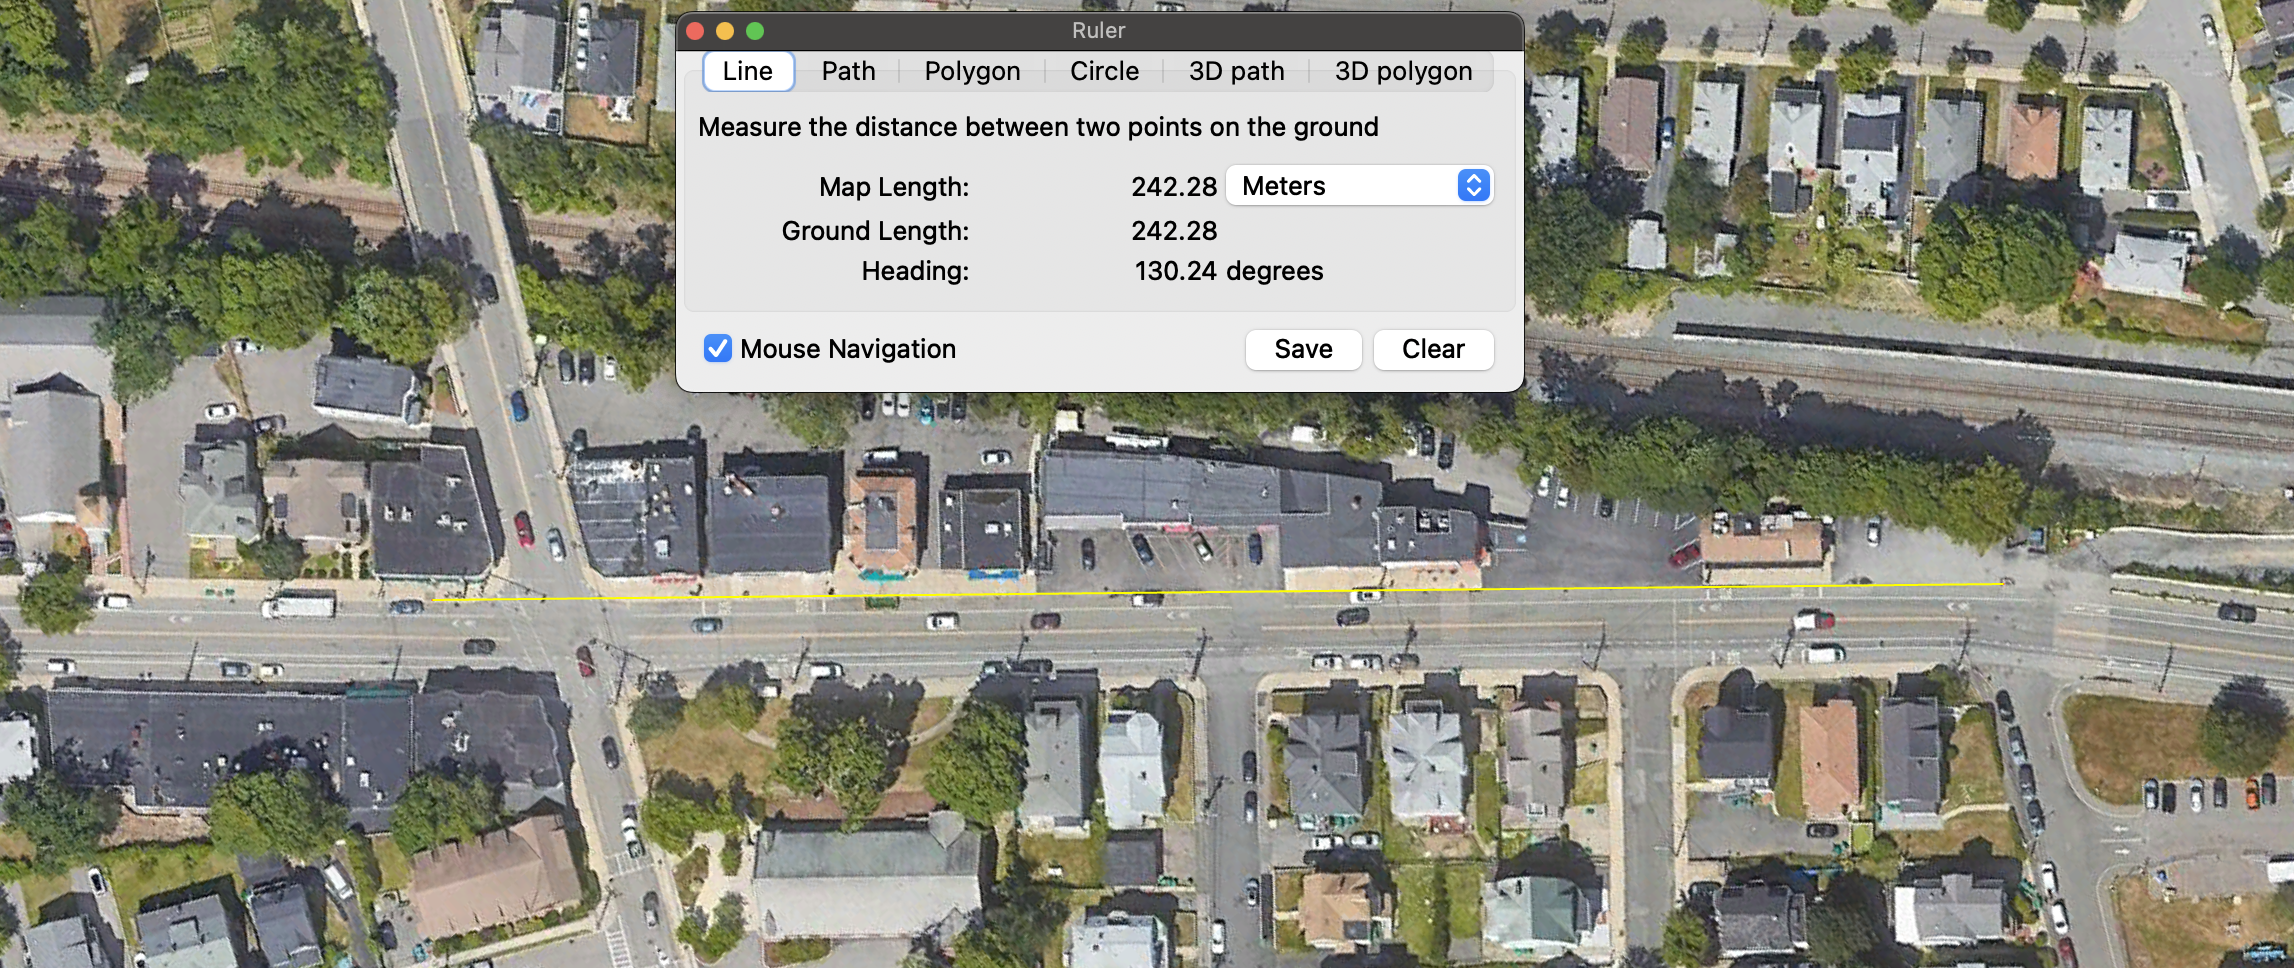
\includegraphics[width=\linewidth]{overleaf/images/range.png}
    \vspace{\ftspace}
    \caption{Approximate Range Test on Boston Avenue, MA}
    \label{fig:range}
\end{figure}

\subsection{\label{sec:res_ping}Ping Response Time}

Do both base ESP-NOW and Networking measurements

\begin{table}[H]
    \centering
    \begin{tabular}{|c|c|}
        \hline
         &  \\
         \hline
         &  \\
         \hline
    \end{tabular}
    \vspace{\ftspace}
    \caption{Ping Response Time}
    \label{tab:ping}
\end{table}

\subsection{\label{sec:res_battery}Battery Test}

As outlined in Section \ref{sec:methods_test_net}, battery life of device was tested.

\subsection{\label{sec:res_reliability}Reliability Test}
A reliability test was done during the first Hackathon which is detailed in Section \ref{sec:methods_hackathon1} and whose results are discussed in Section \ref{sec:res_hackathon1}. As part of this test, over ?? participants used the boop-o-meter to send messages to each other, which was done without any problems.

\subsection{\label{sec:res_rssi}Response Time, RSSI and Packet Loss Rate by Range}

Also include results for experiments for range, rssi and latency.

\begin{table}[H]
    \centering
    \begin{tabular}{|c||c|c|c|c||c|c|c|c|}
        \hline
        & \multicolumn{4}{c||}{\textbf{ESP32C3}} & \multicolumn{4}{c|}{\textbf{ESP32C6}} \\
        \hline\hline
        \multirow{6}{10pt}{\rotatebox{90}{\textbf{ESP32C3}}} & \textbf{Distance} & \textbf{RSSI} & \textbf{Latency} & \textbf{Loss \%} & \textbf{Distance} & \textbf{RSSI} & \textbf{Latency} & \textbf{Loss \%} \\
        \cline{2-9}
        &  &  &  &  &  &  &  &  \\
        \cline{2-9}
        &  &  &  &  &  &  &  &  \\
        \cline{2-9}
        &  &  &  &  &  &  &  &  \\
        \cline{2-9}
        &  &  &  &  &  &  &  &  \\
        \cline{2-9}
        &  &  &  &  &  &  &  &  \\
        \hline
        \hline
        \multirow{6}{10pt}{\rotatebox{90}{\textbf{ESP32C6}}} & \textbf{Distance} & \textbf{RSSI} & \textbf{Latency} & \textbf{Loss \%} & \textbf{Distance} & \textbf{RSSI} & \textbf{Latency} & \textbf{Loss \%} \\
        \cline{2-9}
        &  &  &  &  &  &  &  &  \\
        \cline{2-9}
        &  &  &  &  &  &  &  &  \\
        \cline{2-9}
        &  &  &  &  &  &  &  &  \\
        \cline{2-9}
        &  &  &  &  &  &  &  &  \\
        \cline{2-9}
        &  &  &  &  &  &  &  &  \\
        \cline{1-1}\cline{2-9}
    \end{tabular}
    \vspace{\ftspace}
    \caption{Range, RSSI, Latency and Packet Loss Rate}
    \label{tab:rssi}
\end{table}

\begin{table}[H]
    \centering
    \begin{tabular}{|c|c|l|c|c|c|c|c|}
    \hline
        Range & Packet Loss & Measurement & mean & std & min & max & median \\\hline
        [meters] & [\%] &  &  &  &  &  &  \\\hline\hline
        \multirow{3}{*}{0 m} & \multirow{1}{*}{0} & RSSI 1 [asu] & -6.05 & 1.14 & -12 & -5 & -6 \\\cline{2-8}\cline{2-8}
        %&& Time 1 &  &  &  &  &  \\\cline{2-8}\cline{2-8}
        & \multirow{2}{*}{0} & RSSI 2 [asu] & -5.44 & 0.67 & -8 & -5 & -5 \\\cline{3-8}
        %&& Time 2 &  &  &  &  &  \\\cline{3-8}
        && Ping [ms] & 20.57 & 0.61 & 19 & 23 & 20 \\\hline\hline
        \multirow{3}{*}{0.1 m} & \multirow{1}{*}{0} & RSSI 1 [asu] & -15.5 & 0.59 & -17 & -15 & -15 \\\cline{2-8}\cline{2-8}
        %&& Time 1 &  &  &  &  &  \\\cline{2-8}\cline{2-8}
        & \multirow{2}{*}{0} & RSSI 2 [asu] & -15.25 & 0.54 & -16 & -14 & -15 \\\cline{3-8}
        %&& Time 2 &  &  &  &  &  \\\cline{3-8}
        && Ping [ms] & 20.36 & 1.08 & 19 & 30 & 20 \\\hline\hline
        \multirow{3}{*}{0.25 m} & \multirow{1}{*}{0} & RSSI 1 [asu] & -20.59 & 0.72 & -23 & -20 & -20 \\\cline{2-8}\cline{2-8}
        %&& Time 1 &  &  &  &  &  \\\\cline{2-8}\cline{2-8}
        & \multirow{2}{*}{0} & RSSI 2 [asu] & -20.58 & 0.53 & -22 & -20 & -21 \\\cline{3-8}
        %&& Time 2 &  &  &  &  &  \\\cline{3-8}
        && Ping [ms] & 20.16 & 0.58 & 17 & 21 & 20 \\\hline\hline
        \multirow{3}{*}{0.5 m} & \multirow{1}{*}{0} & RSSI 1 [asu] & -27.22 & 0.73 & -29 & -25 & -27 \\\cline{2-8}\cline{2-8}
        %&& Time 1 &  &  &  &  &  \\\cline{2-8}\cline{2-8}
        & \multirow{2}{*}{0} & RSSI 2 [asu] & -27.15 & 0.77 & -30 & -25 & -27 \\\cline{3-8}
        %&& Time 2 &  &  &  &  &  \\\cline{3-8}
        && Ping [ms] & 23.32 & 22.42 & 19 & 223 & 20 \\\hline\hline
        \multirow{3}{*}{1 m} & \multirow{1}{*}{0} & RSSI 1 [asu] & -31.14 & 0.93 & -33 & -29 & -31 \\\cline{2-8}\cline{2-8}
        %&& Time 1 &  &  &  &  &  \\\cline{2-8}\cline{2-8}
        & \multirow{2}{*}{0} & RSSI 2 [asu] & -31-18 & 0.74 & -29 & -33 & -31 \\\cline{3-8}
        %&& Time 2 &  &  &  &  &  \\\cline{3-8}
        && Ping [ms] & 23.29 & 22.11 & 19 & 219 & 20 \\\hline\hline
        \multirow{3}{*}{5 m} & \multirow{1}{*}{0} & RSSI 1 [asu] & -42.67 & 0.97 & -45 & -41 & -43 \\\cline{2-8}\cline{2-8}
        %&& Time 1 &  &  &  &  &  \\\cline{2-8}\cline{2-8}
        & \multirow{2}{*}{0} & RSSI 2 [asu] & -44.91 & 2.87 & -72 & -42 & -45 \\\cline{3-8}
        %&& Time 2 &  &  &  &  &  \\\cline{3-8}
        && Ping [ms] & 22.47 & 9.34 & 10 & 50 & 20 \\\hline\hline
        \multirow{3}{*}{10 m} & \multirow{1}{*}{0} & RSSI 1 [asu] & -45.03 & 1.23 & -50 & -43 & -45 \\\cline{2-8}\cline{2-8}
        %&& Time 1 &  &  &  &  &  \\\cline{2-8}\cline{2-8}
        & \multirow{2}{*}{0} & RSSI 2 [asu] & -46.83 & 1.01 & -50 & -45 & -47 \\\cline{3-8}
        %&& Time 2 &  &  &  &  &  \\\cline{3-8}
        && Ping [ms] & 19.8 & 7.52 & 10 & 41 & 20 \\\hline\hline
        \multirow{3}{*}{25 m} & \multirow{1}{*}{3} & RSSI 1 [asu] & -62.54 & 3.17 & -87 & -57 & -63 \\\cline{2-8}\cline{2-8}
        %&& Time 1 &  &  &  &  &  \\\cline{2-8}\cline{2-8}
        & \multirow{2}{*}{3} & RSSI 2 [asu] & -64.72 & 2.04 & -71 & -60 & -65 \\\cline{3-8}
        %&& Time 2 &  &  &  &  &  \\\cline{3-8}
        && Ping [ms] & 18.88 & 7.46 & 9 & 41 & 20 \\\hline\hline
        \multirow{3}{*}{50 m} & \multirow{1}{*}{12} & RSSI 1 [asu] & -65.69 & 2.38 & -73 & -62 & -65 \\\cline{2-8}\cline{2-8}
        %&& Time 1 &  &  &  &  &  \\\\cline{2-8}\cline{2-8}
        & \multirow{2}{*}{12} & RSSI 2 [asu] & -68.08 & 2.38 & -74 & -64 & -68 \\\cline{3-8}
        %&& Time 2 &  &  &  &  &  \\\cline{3-8}
        && Ping [ms] & 20.95 & 11.22 & 10 & 91 & 20 \\\hline\hline
        \multirow{3}{*}{100 m} & \multirow{1}{*}{32} & RSSI 1 [asu] & -70.12 & 3.61 & -82 & -63 & -69 \\\cline{2-8}\cline{2-8}
        %&& Time 1 &  &  &  &  &  \\\cline{2-8}\cline{2-8}
        & \multirow{2}{*}{34} & RSSI 2 [asu] & -73-52 & 3.27 & -86 & -66 & -73 \\\cline{3-8}
        %&& Time 2 &  &  &  &  &  \\\cline{3-8}
        && Ping [ms] & 26.29 & 18.17 & 10 & 141 & 20 \\\hline
    \end{tabular}
    \vspace{\ftspace}
    \caption{RSSI, ping time and package loss measurements for various ranges}
    \label{tab:ping_rssi_res}
\end{table}

\subsection{\label{sec:res_angle} Antenna Angle Effects on RSSI and Ping Response Time}

As outlined in Section \ref{sec:methods_test_net}. Experiment at fixed range

\begin{table}[H]
    \centering
    \begin{tabular}{|c|c|l|c|c|c|c|c|}
    \hline
        Angle & Packet Loss & Measurement & mean & std & min & max & median \\\hline
        [\degree] & [\%] &  &  &  &  &  &  \\\hline\hline
        \multirow{3}{*}{$0\degree$} & \multirow{1}{*}{0} & RSSI 1 [asu] & -35.71 & 0.6 & -37 & -35 & -36 \\\cline{2-8}\cline{2-8}
        %&& Time 1 &  &  &  &  &  \\\cline{2-8}\cline{2-8}
        & \multirow{2}{*}{0} & RSSI 2 [asu] & -34.8 & 0.51 & -37 & -35 & -35 \\\cline{3-8}
        %&& Time 2 &  &  &  &  &  \\\cline{3-8}
        && Ping [ms] & 20.2 & 1.53 & 10 & 30 & 20 \\\hline\hline
        \multirow{3}{*}{$45\degree$} & \multirow{1}{*}{0} & RSSI 1 [asu] & -37.74 & 1.47 & -41 & -35 & 38 \\\cline{2-8}\cline{2-8}
        %&& Time 1 &  &  &  &  &  \\\cline{2-8}\cline{2-8}
        & \multirow{2}{*}{0} & RSSI 2 [asu] & -37.47 &1.49 & -40 & -35 & -37 \\\cline{3-8}
        %&& Time 2 &  &  &  &  &  \\\cline{3-8}
        && Ping [ms] & 20.14 & 0.58 & 17 & 21 & 20 \\\hline\hline
        \multirow{3}{*}{$90\degree$} & \multirow{1}{*}{0} & RSSI 1 [asu] & -34.33 & 1.18 & -38 & -33 & -34 \\\cline{2-8}\cline{2-8}
        %&& Time 1 &  &  &  &  &  \\\cline{2-8}\cline{2-8}
        & \multirow{2}{*}{0} & RSSI 2 [asu] & -33.68 & 1.15 & -37 & -32 & -33 \\\cline{3-8}
        %&& Time 2 &  &  &  &  &  \\\cline{3-8}
        && Ping [ms] & 20.08 & 1.12 & 10 & 21 & 20 \\\hline\hline
        \multirow{3}{*}{$135\degree$} & \multirow{1}{*}{0} & RSSI 1 [asu] & -35.12 & 0.72 & -36 & -33 & -35 \\\cline{2-8}\cline{2-8}
        %&& Time 1 &  &  &  &  &  \\\cline{2-8}\cline{2-8}
        & \multirow{2}{*}{0} & RSSI 2 [asu] & -34.64 & 0.7 & -36 & -32 & -35 \\\cline{3-8}
        %&& Time 2 &  &  &  &  &  \\\cline{3-8}
        && Ping [ms] & 20.12 & 0.77 & 14 & 21 & 20 \\\hline\hline
        \multirow{3}{*}{$180\degree$} & \multirow{1}{*}{0} & RSSI 1 [asu] & -37.01 & 0.96 & -39 & -34 & -37 \\\cline{2-8}\cline{2-8}
        %&& Time 1 &  &  &  &  &  \\\cline{2-8}\cline{2-8}
        & \multirow{2}{*}{0} & RSSI 2 [asu] & -36.73 & 0.86 & -39 & -33 & -37 \\\cline{3-8}
        %&& Time 2 &  &  &  &  &  \\\cline{3-8}
        && Ping [ms] & 20.04 & 1.05 & 11 & 21 & 20 \\\hline
    \end{tabular}
    \vspace{\ftspace}
    \caption{RSSI, ping time and package loss measurements for various angles at fixed distance (1 meter)}
    \label{tab:angle_res}
\end{table}

\begin{figure}[H]
    \centering
    \includegraphics[width=0.5\linewidth]{overleaf/images/placeholder.png}
    \vspace{\ftspace}
    \caption{RSSI and Ping Time depending on antenna angle}
    \label{fig:antennaangle}
\end{figure}


\subsection{\label{sec:res_limitations}Limitations}

%Limitations of networking...

Inherit in the system there is no handshake, so if a message is lost, it is lost forever. Conscious decision for this, as if there are no 



\section{\label{sec:res_validation}Validation}

\subsection{\label{sec:res_examplekit}Example Robotics Kit and Showcase}

ehhhhhhhhh, maybe present the three little programs I had written here

\subsection{\label{sec:res_hackathon1}Hackathon 1}

Networking developed and idea gathering on how it could be used.

Result from the hackathon was that it was too complicated to get started, furthermore, the amount of messages sent was overwhelming since everybody was sending to everybody. Most people were not able to build anything useable. 

Main take-away of making it more approachable, include example code and a better guide. This has then lead to the development of development tools.

\subsection{\label{sec:res_hackathon2}Hackathon 2}

Test of development tools and application potential for educational or fun activities.

\subsection{\label{sec:res_honourablementions}Mention of Projects that have used the Platform for Development}

mention playground project which made a lot of use of networking capability

Limitations?
